
\documentclass{article}
\usepackage{amsmath, amssymb, graphicx, hyperref, float}
\usepackage[margin=1in]{geometry}

\title{Dual-Curve Trapdoor Cryptography: A Novel Intersection-Based Hashing Scheme}
\author{[Your Name Here]}
\date{\today}

\begin{document}
\maketitle

\begin{abstract}
This paper introduces a novel cryptographic concept that leverages the intersection of two mathematical curves to generate secure cryptographic outputs. The approach modifies traditional elliptic curve cryptography by introducing a secondary curve and utilizing the coordinates of their intersection, when approached via scalar multiplication from a random generator point. The resulting intersection coordinates are hashed using SHA-256, producing a unique and secure cryptographic hash.
\end{abstract}

\section{Introduction}
Elliptic Curve Cryptography (ECC) has become a cornerstone of modern cryptographic systems due to its efficiency and high level of security relative to key size. This proposal seeks to expand upon the ECC paradigm by introducing a second mathematical function or graph into the cryptographic process. This additional layer of complexity creates a new kind of cryptographic trapdoor function, one based on geometric interaction rather than purely algebraic relations.

\section{Concept Overview}
The core idea involves:
\begin{enumerate}
  \item Selecting a primary elliptic curve:
  \[ E: y^2 = x^3 + ax + b \]
  \item Selecting a secondary curve (arbitrary), such as:
  \begin{itemize}
    \item \( y = \sin(x) \)
    \item \( y = \log(x) \)
    \item Another elliptic curve \( y^2 = x^3 + cx + d \)
  \end{itemize}
  \item Choosing a random generator point \( G \in E \)
  \item Performing scalar multiplication:
  \[ P = k \cdot G \]
  \item Observing when \( P \) intersects the secondary graph
  \item Hashing the coordinates of that point with SHA-256:
  \[ H = \text{SHA-256}(x_P, y_P) \]
\end{enumerate}
This process creates a cryptographic value based on both the algebraic properties of the elliptic curve and the geometric alignment with a second graph.

\section{Visual Representation}
\begin{figure}[H]
\centering
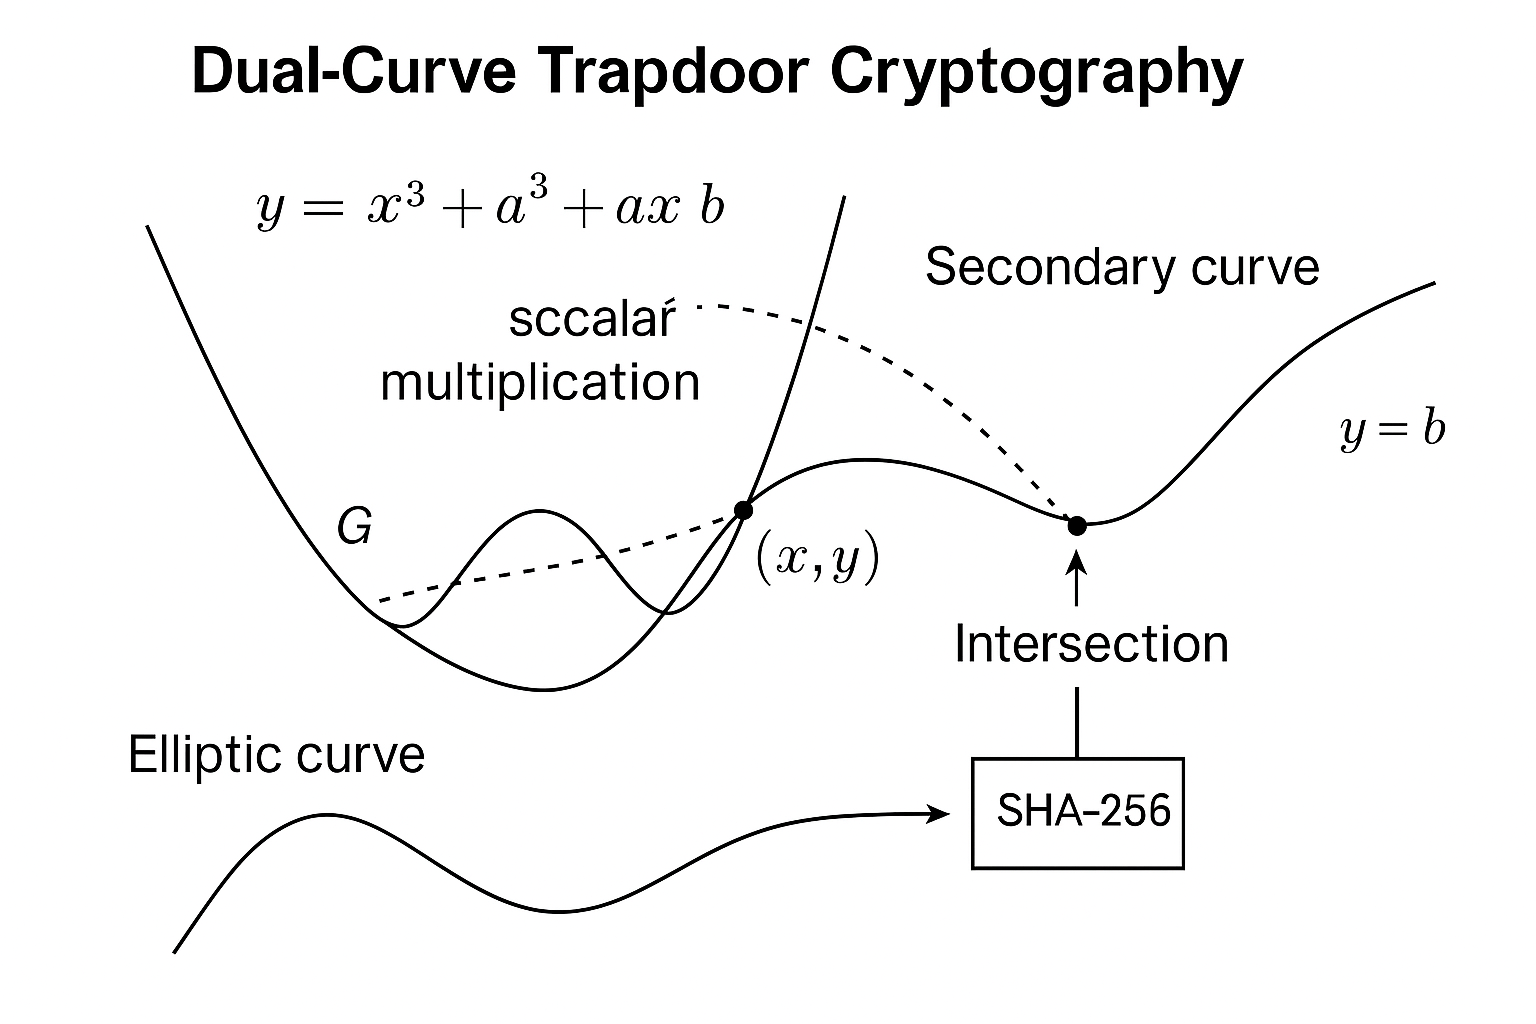
\includegraphics[width=0.85\textwidth]{dual_curve_graph.png}
\caption{A scalar walk across an elliptic curve intersecting a secondary graph (e.g., sine wave). The intersection coordinates are hashed using SHA-256.}
\end{figure}

\section{Security Implications}
\begin{itemize}
  \item \textbf{ECDLP Hardness Preserved:} The use of scalar multiplication retains the hardness of the Elliptic Curve Discrete Logarithm Problem.
  \item \textbf{Increased Entropy:} Random generator point selection and secondary curve behavior introduce unpredictability.
  \item \textbf{Trapdoor Design:} Only entities knowing the correct generator point and curves can recreate the correct hash.
  \item \textbf{Resistance to Brute Force:} The search space is vastly increased due to the dual-curve requirement.
\end{itemize}

\section{Potential Applications}
\begin{itemize}
  \item Advanced Key Derivation Functions (KDFs)
  \item Novel Proof-of-Work Schemes
  \item Secure Hash-Based Message Authentication
  \item Decentralized Identity Systems with Custom Curve Logic
\end{itemize}

\section{Future Work}
\begin{itemize}
  \item Formal mathematical modeling of intersection frequency and randomness.
  \item Exploration of finite-field adaptations.
  \item Development of a protocol or API around this method.
  \item Security analysis under quantum computing assumptions.
\end{itemize}

\section{Conclusion}
This document outlines a novel approach to cryptography that blends scalar multiplication with geometric intersection to produce unpredictable and secure hash values. It represents a new direction for cryptographic exploration, potentially offering strong resistance to future cryptographic threats.

\end{document}
